\documentclass[11pt]{article}
\usepackage[margin=0.8in]{geometry}
\usepackage[T1]{fontenc}
\usepackage[utf8]{inputenc}
\usepackage{booktabs,longtable,graphicx,url,array,microtype}
\setlength{\LTpre}{6pt}
\setlength{\LTpost}{6pt}
\setlength{\tabcolsep}{3pt}
\renewcommand{\arraystretch}{1.08}
\renewcommand{\thetable}{S\arabic{table}}
\renewcommand{\thefigure}{S\arabic{figure}}
\title{Supplementary Material for\\\emph{Timestep-Conditioned Adapter Scaling for Multi-view Diffusion Texture Generation}}
\author{Anonymous authors}
\date{}
\begin{document}
\maketitle
\noindent This supplement supports the revised 01549 manuscript. Fresh C is an image-space comparison on 300 UIDs disjoint from the original 01549 evaluation/probe IDs, the 1,118-object training list, and clean-v2 evaluation IDs. Its primary conditions and same-cohort addendum share one frozen adapter checkpoint, runner source, seed policy, inputs, target views, and metric implementation; the addendum is not an independent replication. Fresh C uses a controlled-retraining checkpoint and is not presented as a numerical reproduction of historical Table 4. Historical cohorts and interface checks are reported separately. Object is the inferential unit; multiple views and wrapper records do not increase $N$.

\section*{S1. Figure asset credits and selection status}
Main Figures~4--5 use Fresh C reference and method-level RGB outputs in a compact context-plus-shared-ROI layout. The original six-view, seven-condition panels, including No Adapter, LLH, and Generic Linear, remain in Supplementary Figure~S1. The selected examples are outcome-ranked illustrations, not a representative sample. Image, checkpoint, run, seed, ROI, and output hashes are listed in \texttt{FRESH\_C\_FIGURE\_SOURCE\_ROI\_MANIFEST.csv}.

The Fresh C No Adapter condition sets the geometry-adapter scale to zero. In the MVPainter wrapper, when \texttt{\_adapter\_scale} is unset the geometry residual is applied without a scale multiplier. These are different settings: No Adapter is not a rendered comparison against the unmodified native-default adapter path. Fresh C contains no separate output for that native-default path, so this part of the R1.1 request remains partially unresolved.

The current rights ledger records the four main-figure assets below as CC Attribution (CC BY 4.0), with figure use allowed when attributed. The complete credit line for each use is:
\begin{longtable}{p{4.3cm}p{10.9cm}}
\caption{Attribution for selected Fresh C assets in main Figures~4--5 and Supplementary Figure~S1.}\label{tab:supp-credits}\\
\toprule Use & Full attribution \\
\midrule\endfirsthead
\toprule Use & Full attribution \\
\midrule\endhead
Figure 4(a), C3--GFL endpoint-favourable example & \emph{Building 03} by Shalmon, via Sketchfab (\url{https://sketchfab.com/3d-models/c76ac44df995482185077da81939b306}), licensed CC BY 4.0 (\url{https://creativecommons.org/licenses/by/4.0/}). Fresh C target-view RGB outputs are cropped to the same ROI and arranged without color or detail adjustment. \\
Figure 5(a), C3-versus-fixed-scale example & \emph{Octaèdre} by Segolene Delamare, via Sketchfab (\url{https://sketchfab.com/3d-models/0571e6db30c84b1593bc55a8e145a430}), licensed CC BY 4.0 (\url{https://creativecommons.org/licenses/by/4.0/}). Fresh C target-view RGB outputs are cropped to the same ROI and arranged without color or detail adjustment. \\
Figure 5(b), Generic Linear counterexample & \emph{Cube 01} by b0rF4x, via Sketchfab (\url{https://sketchfab.com/3d-models/06fa4974f8cd4d4ea792e98fa1521457}), licensed CC BY 4.0 (\url{https://creativecommons.org/licenses/by/4.0/}). Fresh C target-view RGB outputs are cropped to the same ROI and arranged without color or detail adjustment. \\
Figure 4(b) and Figure S1(a), adverse C3--GFL example & \emph{Boat Low Poly Game Ready} by INinja, via Sketchfab (\url{https://sketchfab.com/3d-models/d0e116a62bfc4cdd9edf60671073b306}), licensed CC BY 4.0 (\url{https://creativecommons.org/licenses/by/4.0/}). Fresh C target-view RGB outputs are cropped to the same ROI and arranged without color or detail adjustment. \\
Figure S1(b), color/detail mismatch example & \emph{E5-5-2} by artsiyu, via Sketchfab (\url{https://sketchfab.com/3d-models/f6979d7ff8e54c4daf00fee46f09a139}), licensed CC BY 4.0 (\url{https://creativecommons.org/licenses/by/4.0/}). The complete Fresh C contact sheet is retained for a broader-condition comparison. \\
\bottomrule
\end{longtable}

\section*{S2. Complete Fresh C paired image-space statistics}
Table~\ref{tab:supp-freshc} reports the complete seven-endpoint paired results for C3--GFL and each of the three named addendum contrasts. The primary C3--GFL FG-PSNR result is unadjusted as the single registered primary endpoint. The six registered secondary C3--GFL endpoints use their Holm family. The addendum's FG-PSNR and FG-LPIPS contrasts use the frozen six-test primary family; the other five endpoints per contrast use the separate 15-test secondary Core-7 family. All contrasts are mean A-minus-B differences with 10,000 object bootstrap resamples and pointwise two-sided percentile 95\% CIs. Positive values favour A for PSNR/SSIM; negative values favour A for LPIPS. Adjusted $p$-values are from the frozen analysis authority. “A favourable” is the fraction of object-level differences in A's favourable direction and is descriptive.

\begingroup\scriptsize
\begin{longtable}{p{2.5cm}p{4.0cm}p{1.5cm}p{1.5cm}p{1.6cm}}
\caption{Complete paired object-level image-space results for the primary C3--GFL contrast and the three named same-cohort addendum contrasts. Differences are A minus B; favorable-object percentages respect endpoint direction.}\label{tab:supp-freshc}\\
\toprule
Endpoint & Mean difference [95\% CI] & Median & A favorable & Adjusted $p$ \\
\midrule
\endfirsthead
\toprule Endpoint & Mean difference [95\% CI] & Median & A favorable & Adjusted $p$ \\
\midrule\endhead
\multicolumn{5}{l}{\textbf{C3 minus GFL}}\\
FG-PSNR (dB) & +0.522 [+0.404, +0.641] & +0.555 & 68.7\% & primary \\
FG-LPIPS & -0.005345 [-0.006326, -0.004403] & -0.004547 & 71.0\% & $3.2\times 10^{-22}$ \\
FG-SSIM & +0.02453 [+0.02120, +0.02805] & +0.02004 & 84.3\% & $5.9\times 10^{-33}$ \\
Edge-SSIM & +0.004494 [+0.003411, +0.005586] & +0.003613 & 69.0\% & $9.4\times 10^{-14}$ \\
Full-view PSNR (dB) & +0.271 [+0.170, +0.373] & +0.220 & 59.3\% & $4\times 10^{-07}$ \\
Full-view LPIPS & -0.003880 [-0.004926, -0.002873] & -0.003029 & 64.3\% & $8\times 10^{-13}$ \\
Full-view SSIM & +0.005619 [+0.004627, +0.006704] & +0.005205 & 83.0\% & $7.9\times 10^{-22}$ \\
\multicolumn{5}{l}{\textbf{C3 minus Generic Linear}}\\
FG-PSNR (dB) & -0.593 [-0.837, -0.351] & +0.074 & 51.7\% & $7.2\times 10^{-06}$ \\
FG-LPIPS & +0.013512 [+0.011601, +0.015487] & +0.012229 & 25.7\% & $1.3\times 10^{-32}$ \\
FG-SSIM & -0.02810 [-0.03197, -0.02439] & -0.02521 & 20.0\% & $2.9\times 10^{-35}$ \\
Edge-SSIM & -0.010693 [-0.013004, -0.008495] & -0.008967 & 33.7\% & $1.6\times 10^{-17}$ \\
Full-view PSNR (dB) & -0.503 [-0.686, -0.322] & -0.139 & 46.7\% & $2.7\times 10^{-07}$ \\
Full-view LPIPS & -0.000897 [-0.002578, +0.000862] & -0.001307 & 54.3\% & $0.611$ \\
Full-view SSIM & +0.000046 [-0.000984, +0.001011] & +0.001213 & 57.0\% & $0.927$ \\
\multicolumn{5}{l}{\textbf{LLH minus C3}}\\
FG-PSNR (dB) & +0.621 [+0.391, +0.855] & -0.153 & 46.7\% & $1.2\times 10^{-06}$ \\
FG-LPIPS & -0.012140 [-0.013861, -0.010480] & -0.010837 & 75.0\% & $9\times 10^{-34}$ \\
FG-SSIM & +0.01658 [+0.01311, +0.02003] & +0.01307 & 67.0\% & $9\times 10^{-18}$ \\
Edge-SSIM & +0.009033 [+0.006867, +0.011296] & +0.006741 & 63.3\% & $2.3\times 10^{-13}$ \\
Full-view PSNR (dB) & +0.816 [+0.639, +0.998] & +0.419 & 59.3\% & $3.2\times 10^{-16}$ \\
Full-view LPIPS & +0.004909 [+0.003266, +0.006510] & +0.004538 & 36.7\% & $3.5\times 10^{-08}$ \\
Full-view SSIM & -0.004330 [-0.005176, -0.003482] & -0.004563 & 27.7\% & $5.9\times 10^{-20}$ \\
\multicolumn{5}{l}{\textbf{LLH minus Generic Linear}}\\
FG-PSNR (dB) & +0.028 [-0.015, +0.070] & +0.017 & 52.3\% & $0.201$ \\
FG-LPIPS & +0.001372 [+0.000762, +0.002081] & +0.000176 & 46.7\% & $0.000114$ \\
FG-SSIM & -0.01152 [-0.01337, -0.00996] & -0.00945 & 8.0\% & $2.6\times 10^{-31}$ \\
Edge-SSIM & -0.001660 [-0.002096, -0.001256] & -0.001648 & 27.3\% & $1.2\times 10^{-12}$ \\
Full-view PSNR (dB) & +0.313 [+0.278, +0.347] & +0.304 & 87.3\% & $2\times 10^{-47}$ \\
Full-view LPIPS & +0.004011 [+0.003390, +0.004684] & +0.003904 & 18.0\% & $1.7\times 10^{-26}$ \\
Full-view SSIM & -0.004284 [-0.005217, -0.003543] & -0.003432 & 5.7\% & $8.5\times 10^{-20}$ \\
\bottomrule
\end{longtable}

\endgroup

\section*{S3. Supporting layer/window and schedule evidence}
A2 is exploratory discovery evidence; A3 is a higher-dose stress regime on the same underlying cohort. A3b is a bounded Fresh B layer/window analysis. Object-cluster tests detect response heterogeneity under the tested interventions, but they do not identify a dose-independent layer-by-time mechanism or an optimal schedule.

\begin{table}[ht]
\centering\small
\caption{Object-cluster Wald interaction summaries for the tested layer-by-window maps. Cell RMSE and interaction share describe these observed maps; they are not causal effect sizes.}\label{tab:supp-layerwindow}
\begin{tabular}{lp{2.1cm}rp{4.2cm}p{2.6cm}}\toprule Map & Endpoint & Wald statistic & Interaction share; cell RMSE & Wald $p$ (A3b Holm) \\\midrule
A2 & FG-LPIPS & 481.081 & 43.5\%; 0.001695 & $8.04\times10^{-99}$ \\
A2 & FG-PSNR & 1879.963 & 56.8\%; 0.1222 dB & $<10^{-300}$ \\
A3 & FG-LPIPS & 657.237 & 11.9\%; 0.00643 & $1.14\times10^{-136}$ \\
A3 & FG-PSNR & 1389.118 & 0.8\%; 0.207 dB & $1.28\times10^{-294}$ \\
A3b & FG-LPIPS & 225.015 & 14.0\%; 0.000342 & $5.37\times10^{-43}$ \\
A3b & FG-PSNR & 525.700 & 36.0\%; 0.0205 dB & $3.43\times10^{-107}$ \\
\bottomrule\end{tabular}
\end{table}

For A3b, the three layer groups had no common support across 2,250 layer-step rows. Their central 90\% realized-dose ranges were deep 56,359--79,927, middle 11,421--19,336, and shallow 2,816--5,193. Dose-adjusted extrapolations do not supply the missing common support. These results therefore support only measurable response heterogeneity under the tested intervention regime.

The separate Fresh B cohort ($N=150$) supplies schedule-location context for LLH, not evidence for C3. Table~\ref{tab:supp-freshb} preserves both registered LLH comparisons and the post-outcome HLL--LLL diagnostic. Paired intervals use 10,000 object-bootstrap resamples (seed 20261002). The LLH--LFM-EXACT intervals lie within the protocol's practical margins (FG-PSNR $\pm0.5$ dB; FG-LPIPS $\pm0.01$); this is a budget-explained interpretation within those margins, not exact equality. HLL--LLL is exploratory and its endpoint directions differ.

The Fresh B protocol-lock file states a freeze time of 2026-10-05 08:40 UTC, while the earliest preserved commit containing that file is dated 2026-10-06 00:52 UTC; its parent does not contain the file. This history does not establish when the lock was first created outside Git, but it cannot authenticate pre-run availability. Accordingly, Fresh B temporal contrasts, the A3b map, and the post-lock generic extension are treated as retrospective sensitivity evidence in this paper, even where their calculations follow the recorded comparison family. They are not described as verified preregistered confirmation.

\begin{table}[ht]
\centering\small
\caption{Fresh B paired object-level LLH comparisons, classified here as retrospective sensitivity because pre-run lock availability cannot be authenticated from the preserved history. Effects are A minus B; favorable rates respect endpoint direction. Holm values reproduce the recorded family.}\label{tab:supp-freshb}
\begin{tabular}{p{3.7cm}p{1.7cm}p{5.7cm}p{1.4cm}p{2.2cm}}\toprule Contrast & Endpoint & Mean [95\% CI] & A favors & $p$ / status \\\midrule
LLH--LFM-EXACT & FG-PSNR & +0.325 [+0.209,+0.446] dB & 54.0\% & raw $\leq0.0001$ \\
LLH--LFM-EXACT & FG-LPIPS & $-0.00460$ [$-0.00563,-0.00357$] & 76.0\% & raw $\leq0.0001$ \\
LLH--HLL & FG-PSNR & +0.687 [+0.404,+0.981] dB & 45.3\% & $\leq0.0004$; median $-0.104$ dB \\
LLH--HLL & FG-LPIPS & $-0.01098$ [$-0.01349,-0.00851$] & 80.7\% & $\leq0.0004$ \\
LLH--LLL & FG-PSNR & +0.734 [+0.597,+0.875] dB & 79.3\% & $\leq0.0004$ \\
LLH--LLL & FG-LPIPS & $-0.00845$ [$-0.01029,-0.00659$] & 82.0\% & $\leq0.0004$ \\
HLL--LLL (exploratory) & FG-PSNR & +0.047 [$-0.120,+0.208$] dB & 66.0\% & 0.5696; median +0.476 dB \\
HLL--LLL (exploratory) & FG-LPIPS & +0.00253 [+0.00155,+0.00354] & 40.0\% & $\leq0.0002$; median +0.00139 \\
\bottomrule\end{tabular}
\end{table}

The post-lock generic-schedule extension on this same Fresh B cohort is a retrospective sensitivity analysis, not independent confirmation. Table~\ref{tab:supp-generic} reports the recorded budget-matched comparisons and endpoint-matched linear counter-result. Nominal requested-scale means do not equalize post-scale residual dose; these LLH comparisons do not establish dose-adjusted schedule superiority or strengthen C3 specifically.

\begingroup\scriptsize
\begin{longtable}{p{3.4cm}p{1.7cm}p{4.4cm}p{1.3cm}p{2.4cm}}
\caption{Post-lock Fresh B generic-schedule extension (same $N=150$ cohort). Effects are LLH minus comparator. Budget-matched schedules form the locked eight-schedule family; endpoint-matched linear is the registered counter-comparison.}\label{tab:supp-generic}\\
\toprule Contrast & Endpoint & Mean [95\% CI] & A favors & Holm $p$ \\
\midrule\endfirsthead
\toprule Contrast & Endpoint & Mean [95\% CI] & A favors & Holm $p$ \\
\midrule\endhead
LLH--budget linear & FG-PSNR & +0.0967 [+0.0594,+0.1357] dB & 65.3\% & Holm $p\leq0.0008$ \\
LLH--budget linear & FG-LPIPS & -0.0009 [-0.0013,-0.0004] & 65.3\% & Holm $p=0.0008$ \\
LLH--budget cosine & FG-PSNR & +0.4629 [+0.3526,+0.5780] dB & 74.7\% & Holm $p\leq0.0008$ \\
LLH--budget cosine & FG-LPIPS & -0.0059 [-0.0071,-0.0046] & 80.0\% & Holm $p\leq0.0008$ \\
LLH--budget trapezoid & FG-PSNR & +0.4404 [+0.3334,+0.5521] dB & 74.0\% & Holm $p\leq0.0008$ \\
LLH--budget trapezoid & FG-LPIPS & -0.0057 [-0.0070,-0.0045] & 78.0\% & Holm $p\leq0.0008$ \\
LLH--budget Gaussian & FG-PSNR & +0.4711 [+0.3584,+0.5892] dB & 74.7\% & Holm $p\leq0.0008$ \\
LLH--budget Gaussian & FG-LPIPS & -0.0058 [-0.0071,-0.0045] & 79.3\% & Holm $p\leq0.0008$ \\
LLH--endpoint linear & FG-PSNR & -0.0373 [-0.0829,+0.0086] dB & -- & Holm $p=0.1150$ \\
LLH--endpoint linear & FG-LPIPS & +0.00109 [+0.0004,+0.0019] & -- & Holm $p=0.0024$ \\
\bottomrule
\end{longtable}
\endgroup

\clearpage
\section*{S4. Requested/applied scale and residual-correction accounting}
Table~\ref{tab:supp-execution} lists representative Fresh C C3 records at five denoising steps. The native caps are 3.0 (deep), 3.5 (middle), and 0.8 (shallow). A cap-active fraction of 100\% means all logged records in that group/step were clipped. The applied correction norm is computed after applying the effective scale and depends on the residual itself; it is a logged implementation quantity, not an independent dose or quality outcome. The 750-row source accounting table contains all 50 steps, three groups, and five strategies.

\begingroup\scriptsize
\begin{longtable}{c l c c c r}
\caption{Representative Fresh C requested/applied scale and post-scale residual-correction accounting. Median correction norms are descriptive log summaries over implementation records; wrappers, objects, and timesteps are not independent experimental units.}\label{tab:supp-execution}\\
\toprule Step & Layer group & Requested & Applied & Cap active & Median correction $L_2$ \\
\midrule\endfirsthead
\toprule Step & Layer group & Requested & Applied & Cap active & Median correction $L_2$ \\
\midrule\endhead
0 & Deep & 1.25 & 1.25 & 0\% & 1309.19 \\
0 & Middle & 1.25 & 1.25 & 0\% & 468.97 \\
0 & Shallow & 1.25 & 0.80 & 100\% & 30.86 \\
12 & Deep & 1.25 & 1.25 & 0\% & 1238.42 \\
12 & Middle & 1.25 & 1.25 & 0\% & 661.91 \\
12 & Shallow & 1.25 & 0.80 & 100\% & 42.79 \\
24 & Deep & 2.50 & 2.50 & 0\% & 2006.94 \\
24 & Middle & 2.50 & 2.50 & 0\% & 1551.26 \\
24 & Shallow & 2.50 & 0.80 & 100\% & 52.51 \\
37 & Deep & 1.25 & 1.25 & 0\% & 672.23 \\
37 & Middle & 1.25 & 1.25 & 0\% & 631.83 \\
37 & Shallow & 1.25 & 0.80 & 100\% & 55.62 \\
49 & Deep & 1.25 & 1.25 & 0\% & 659.98 \\
49 & Middle & 1.25 & 1.25 & 0\% & 197.82 \\
49 & Shallow & 1.25 & 0.80 & 100\% & 34.72 \\
\bottomrule
\end{longtable}

\endgroup

\section*{S5. Historical and cross-interface boundaries}
The completed \texttt{MAIN-STAGE-276} follow-up contains 1,104 records (276 objects by four schedules), with 50 Euler steps, seed 42, unique-six target views, shared initial latents, and a common runner within the run. Its final run manifest records completion with exit code 0. The follow-up was specified after inspection of earlier clean-v2 results and was not blind. It is reported separately from Fresh C and is not an independent replication of the original 01549 development probe.

Here, temporal L--L--H means that the requested values are low in early and middle steps and high in late steps. This is distinct from the layer-conditioned Fresh C LLH addendum condition described in the main paper. With 50 steps, the code assigns 17/16/17 steps to early/middle/late. C3 therefore has deep/middle applied-scale sums of 82.5; temporal L--L--H has 83.75 because its high stage occupies 17 rather than 16 steps; the shallow applied sum is 40 for both after the 0.8 cap. The fixed-mean comparator has a deep/middle sum of 83.33 and a shallow sum of 40. These are near-matched scalar sums, not exactly equal sums or matched residual-norm doses.

Table~\ref{tab:supp-stage-placement} gives all six formal paired endpoints for C3 versus temporal L--L--H and C3 versus the fixed-mean comparator. Effects are C3 minus comparator; positive values favor C3 for PSNR/SSIM, and negative values favor C3 for LPIPS. Temporal L--L--H outperforms C3 on all six formal endpoints in this post-inspection stage-placement experiment: it has higher PSNR/SSIM and lower LPIPS endpoints. In contrast, C3 exceeds fixed-mean on five of six formal endpoints. These results show that the measured response varies with tested stage placement; they do not establish a universal schedule winner. The contrasts do not isolate placement from the small applied-scale-sum differences or the resulting residual-state trajectory, and post-scale residual norms are not matched.

\begin{longtable}{p{3.0cm}p{2.6cm}p{5.8cm}}
\caption{Formal paired comparisons from the strict-276 stage-placement follow-up. Effects are C3 minus comparator; 95\% percentile-bootstrap intervals are object-level.}\label{tab:supp-stage-placement}\\
\toprule Contrast & Endpoint & Mean difference [95\% CI] \\
\midrule\endfirsthead
\toprule Contrast & Endpoint & Mean difference [95\% CI] \\
\midrule\endhead
\multicolumn{3}{l}{\textbf{C3 minus temporal L--L--H}}\\
 & Full-view PSNR (dB) & $-0.268100$ [$-0.311101,-0.227797$] \\
 & FG-PSNR (dB) & $-0.177084$ [$-0.230539,-0.130784$] \\
 & FG-SSIM & $-0.008851$ [$-0.011455,-0.006291$] \\
 & Edge-SSIM & $-0.035301$ [$-0.036581,-0.034031$] \\
 & FG-LPIPS & $+0.001896$ [$+0.001205,+0.002578$] \\
 & Full-view LPIPS & $+0.008658$ [$+0.007465,+0.009831$] \\
\multicolumn{3}{l}{\textbf{C3 minus fixed-mean}}\\
 & Full-view PSNR (dB) & $+0.556369$ [$+0.525520,+0.589220$] \\
 & FG-PSNR (dB) & $+0.502875$ [$+0.462018,+0.542244$] \\
 & FG-SSIM & $+0.032083$ [$+0.028966,+0.035172$] \\
 & Edge-SSIM & $+0.001696$ [$+0.000611,+0.002782$] \\
 & FG-LPIPS & $-0.003797$ [$-0.004341,-0.003260$] \\
 & Full-view LPIPS & $+0.001420$ [$+0.000778,+0.002072$] \\
\bottomrule
\end{longtable}

The saved-artifact Full-SSIM branch is kept separate from the formal pre-save metrics above: C3 minus temporal L--L--H is $-0.001697$ (95\% CI [$-0.002047,-0.001340$]); C3 minus fixed-mean is $+0.007486$ ([$+0.006736,+0.008262$]). These saved-artifact values are not pooled with the formal metric column.

A retrospective strict-276 Core-7 summary uses the clean-v2 object list (SHA-256 \texttt{a6aa8ab6\allowbreak{}e475763e\allowbreak{}1b5e67dc\allowbreak{}8c712ec8\allowbreak{}f1940e39\allowbreak{}52d65897\allowbreak{}c8208875\allowbreak{}54bbd044}) and the same recorded checkpoint SHA as Fresh C. It shares the 276-object cohort/checkpoint lineage with the separate \texttt{MAIN-STAGE-276} profile-placement follow-up, so those results are not independent cohort replications. The row audit verifies 276 unique object indices per condition and identical object labels by index. However, Core-7 does not establish one common runner or fully shared inputs across all seven conditions: No Adapter and GFH are the two newly rerun arms with per-object input-tensor hashes; their recorded runner hash is \texttt{ae5d5664\allowbreak{}e7d0ebcd\allowbreak{}4bd84c7c\allowbreak{}7d688c4a\allowbreak{}8962c6d7\allowbreak{}4463fe88\allowbreak{}e7a86640\allowbreak{}4911e7e0}. C3 records a different runner hash, \texttt{d4af0c1d\allowbreak{}7f42168a\allowbreak{}585b505a\allowbreak{}6d775ea3\allowbreak{}ff7ffb18\allowbreak{}345156eb\allowbreak{}f358f272\allowbreak{}025fa7f2}; GFL and the three layer conditions do not establish the same runner hash, and their serialized rows do not contain per-object input-tensor hashes. Thus Core-7 is a retrospective diagnostic, not a same-runner confirmatory comparison. It is not pooled with Fresh C, and the shared checkpoint hash does not make it a numerical reproduction of the original 01549 Table 4 result.

Table~\ref{tab:supp-core7-means} gives the seven-condition means for the requested image-space endpoints. These stored metrics show an endpoint trade-off: C3 has a higher Full-view PSNR mean than GFH but a lower FG-PSNR mean. The Core-7 Layer LLH row is distinct from Fresh C's layer-conditioned LLH addendum and Fresh B's temporal LLH condition. Table~\ref{tab:supp-core7-contrasts} reports selected object-indexed contrasts. C3--GFH intervals were recalculated from the serialized per-object rows after inspection of the Core-7 summary; they are post-hoc, nominal pointwise intervals. The other listed contrasts reproduce the separate Core-7 paired-statistics file. The intervals describe the saved metric rows and do not overcome the common-runner/input-hash limitations.

\begin{table}[ht]
\centering\scriptsize\setlength{\tabcolsep}{4pt}
\caption{Retrospective Core-7 strict-276 condition means. Rows contain 276 object-level metrics per condition. The collection has incomplete common runner/input identity as described above; means are descriptive and are not Fresh C or an independently verified same-runner comparison.}
\label{tab:supp-core7-means}
\begin{tabular}{lccccc}\toprule
Condition & Full-view PSNR$\uparrow$ & FG-PSNR$\uparrow$ & FG-LPIPS$\downarrow$ & FG-SSIM$\uparrow$ & Edge-SSIM$\uparrow$ \\
\midrule
No Adapter & 10.563 & 8.826 & 0.2059 & 0.4799 & 0.4794 \\
GFL & 18.229 & 10.731 & 0.1917 & 0.3987 & 0.5201 \\
GFH & 18.242 & 13.153 & 0.1677 & 0.4783 & 0.5538 \\
C3 & 18.968 & 11.939 & 0.1817 & 0.4296 & 0.5278 \\
Layer Fixed Mean & 19.516 & 13.100 & 0.1698 & 0.4550 & 0.5363 \\
Layer LHL & 19.635 & 12.974 & 0.1719 & 0.4445 & 0.5273 \\
Layer LLH & 20.828 & 13.975 & 0.1610 & 0.4620 & 0.5476 \\
\bottomrule\end{tabular}
\end{table}

\begin{table}[ht]
\centering\small
\caption{Selected retrospective Core-7 paired contrasts (first condition minus second). Intervals are pointwise 95\% object-bootstrap percentile intervals with 10,000 resamples and seed 20260930; they are unadjusted and descriptive. The C3--GFH intervals were recalculated post hoc. The final column counts objects where the first condition is favorable for PSNR.}
\label{tab:supp-core7-contrasts}
\begin{tabular}{llcc}\toprule
Contrast & Endpoint & Mean difference [95\% CI] (dB) & Objects favoring first \\
\midrule
C3--GFH & Full-view PSNR & $+0.725229$ [$+0.647134,+0.806467$] & 240/276 \\
C3--GFH & FG-PSNR & $-1.214235$ [$-1.313952,-1.114705$] & 25/276 \\
C3--GFL & FG-PSNR & $+1.207771$ [$+1.116967,+1.294989$] & 259/276 \\
LLH--GFH & FG-PSNR & $+0.822292$ [$+0.616795,+1.033035$] & 148/276 \\
LLH--C3 & FG-PSNR & $+2.036527$ [$+1.806804,+2.260756$] & 227/276 \\
\bottomrule\end{tabular}
\end{table}

The frozen MV-Adapter probe analyzed 98 of 99 planned objects; the omitted input was a frozen GLB with path geometry and no triangle faces, so no substitute was used. The production additive-residual bootstrap interaction statistic is retained in the source audit but its null distribution is centered at or above the observed statistic; this test is invalid for interaction inference. The post hoc exploratory object-cluster robust Wald reanalysis uses 8 degrees of freedom and gives FG-LPIPS $W=13.322$, raw $p=0.101$, Holm $p=0.303$; PSNR $W=7.995$, raw $p=0.434$, Holm $p=0.868$; FG-SSIM $W=16.243$, raw $p=0.039$, Holm $p=0.156$; and CIEDE2000 $W=3.945$, raw and Holm $p=0.862$. No metric survives the exploratory four-metric correction. Small adverse shallow FG-LPIPS changes occur in late windows W3--W5 within the registered 15-cell family; the tested scale range may be too weak to reveal larger responses. This bounded, exploratory result does not establish absence of interaction or equivalence. MVDiffusion was evaluated separately on 75 objects using a different correspondence-aware conditioning interface; its within-interface results were mixed/negative across structure, color, and texture endpoints. Neither interface is a matched architecture comparison, so these analyses do not establish architecture causality or cross-backbone generalization. Each system uses its own conditioning and runner, and the measurements are reported within interface rather than as a controlled shared-checkpoint comparison.

The first-round 01549 Section~4.7 adapter-dependence analysis is retained as a separate within-family result. It reported three outcomes for uniform high scale across adapter regimes: texture flattening without per-layer caps, high-frequency artifact amplification under a strong-residual adapter with per-layer caps, and negligible effect for a weakened adapter. Its same-checkpoint cap ablation reported both flattening and amplification, and its residual-magnitude sweep (0.1$\times$--3$\times$ output projection) reported increasing intervention strength with residual magnitude. A six-object stage ablation reported that the most sensitive stage differed between the main and artifact-prone adapters. These first-round results were explicitly described as adapter-dependent; they are retained as historical, within-architecture evidence and do not answer the current cross-backbone question.

A separate 76-object MV-Adapter study tested layer-wise L--LLH under an alternative budget-neutral contiguous partition B$'$ (per-point multipliers $[0.52018,0.52018,1.47982,1.47982]$, weighted mean 1). Relative to the corresponding global controls, the B$'$ results are mixed across endpoints: the layer condition favors the global controls on FG-SSIM, favors the layer condition on the benefit-oriented CIEDE2000 and GT-relative texture summaries, and does not separate on FG-PSNR, Edge-SSIM, or FG-LPIPS. Its difference from the original partition is not resolved on any reported metric. These data describe this MV-Adapter layer intervention only and are not evidence for the TCAS timestep profile or for a general mapping rule.

The companion M3 profile uses $[0.41953,0.41953,1.19349,1.19349]$, whose mean multiplier is approximately 0.8065. It changes both group assignment and total nominal residual budget, so it is not a pure mapping comparison with B$'$. Its audit classified 16 of 18 direction summaries as stable relative to the original partition, with one small Edge-SSIM attenuation and one near-zero FG-LPIPS sign change. Because the preserved protocol and result rows first appear in the same commit, M3 is retained as retrospective sensitivity. Neither M3 nor B$'$ establishes mapping robustness or cross-backbone generalization.

\section*{S6. Historical N=20 unseen-view results}
Table~\ref{tab:supp-n20} reports the bounded historical N=20 GLB results. The subset comprises 20 UV-compatible objects from the original 24-object pool; four inputs were excluded for lack of UVs. Each object is the paired unit after averaging 11 frozen unseen views. Rendering uses unlit base color with native sampler interpretation. Endpoint directions are mixed; these statistics do not establish population-level 3D superiority, PBR/material fidelity, seam quality, or human preference. The source GLB assets and internal montage are not included in this supplement.
\begin{table}[ht]
\centering\small
\caption{Historical N=20 unlit base-color paired unseen-view summaries (C3 minus comparator). The 20-object UV-compatible subset comes from the historical 24-object pool; four objects were excluded for missing UVs. Each object is averaged over 11 frozen unseen views. Intervals are 10,000-object-bootstrap percentile CIs (seed 20261005), descriptive and unadjusted.}\label{tab:supp-n20}
\begin{tabular}{llcc}\toprule Comparator & Endpoint & Mean difference [95\% CI] & Objects favoring C3 \\\midrule
GFL & FG-PSNR (dB) & -0.066 [-0.413, +0.290] & 5/20 (25\%) \\
GFL & FG-LPIPS & -0.004719 [-0.007504, -0.002544] & 17/20 (85\%) \\
GFL & CIEDE2000 & +0.133 [-1.161, +1.319] & 6/20 (30\%) \\
GFH & FG-PSNR (dB) & +0.084 [-0.290, +0.426] & 14/20 (70\%) \\
GFH & FG-LPIPS & +0.007709 [+0.004230, +0.012101] & 4/20 (20\%) \\
GFH & CIEDE2000 & -1.027 [-2.224, +0.229] & 14/20 (70\%) \\
No Adapter & FG-PSNR (dB) & +3.135 [+1.721, +4.493] & 18/20 (90\%) \\
No Adapter & FG-LPIPS & -0.014519 [-0.029860, -0.001326] & 16/20 (80\%) \\
No Adapter & CIEDE2000 & -12.508 [-18.556, -6.529] & 18/20 (90\%) \\
\bottomrule\end{tabular}
\end{table}

\section*{S7. Selected negative visual evidence and unresolved 3D checks}
Figure~\ref{fig:supp-failures} presents selected illustrative Fresh C failure cases. Panel (a) is an object-level case where GFL favours C3 on the paired image-space comparison. Panel (b) illustrates a color/detail mismatch and repeated pattern in the No Adapter output; it is not a C3-specific failure claim. Neither panel estimates failure prevalence. Full attributions appear in Table S1.

\begin{figure}[ht]
\centering
\small\textbf{(a) Selected C3--GFL adverse example}\par\vspace{2pt}
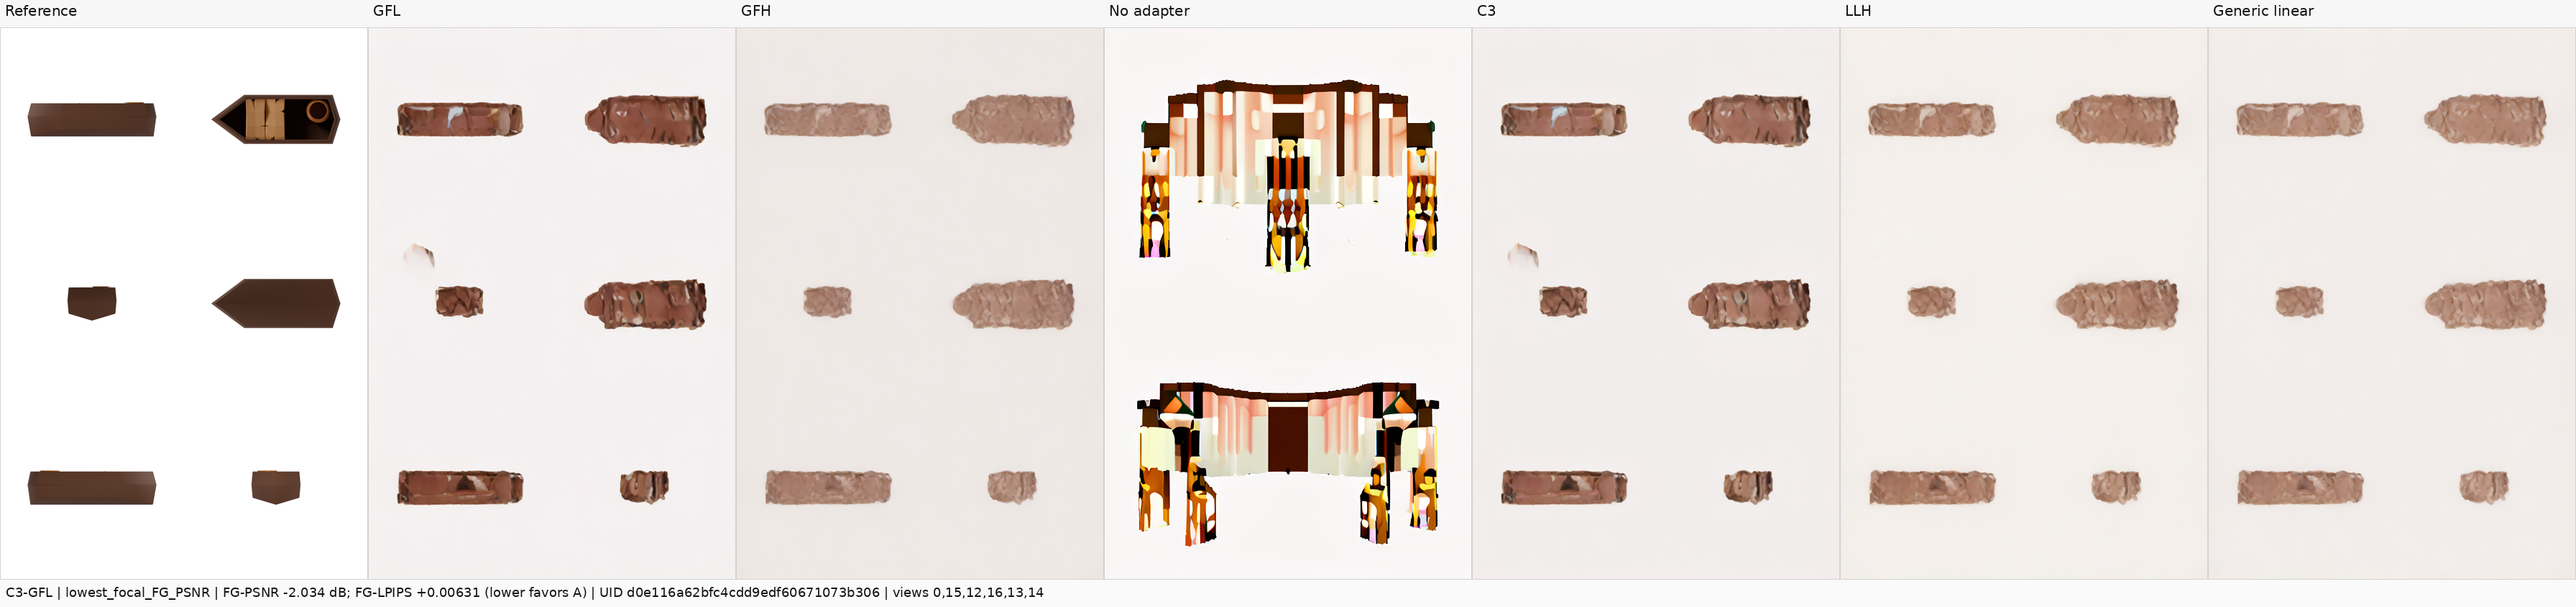
\includegraphics[width=\textwidth,trim=0 36pt 0 0,clip]{figures/figS1_adverse_c3_gfl.png}\par\vspace{5pt}
\small\textbf{(b) Selected color/detail mismatch example}\par\vspace{2pt}
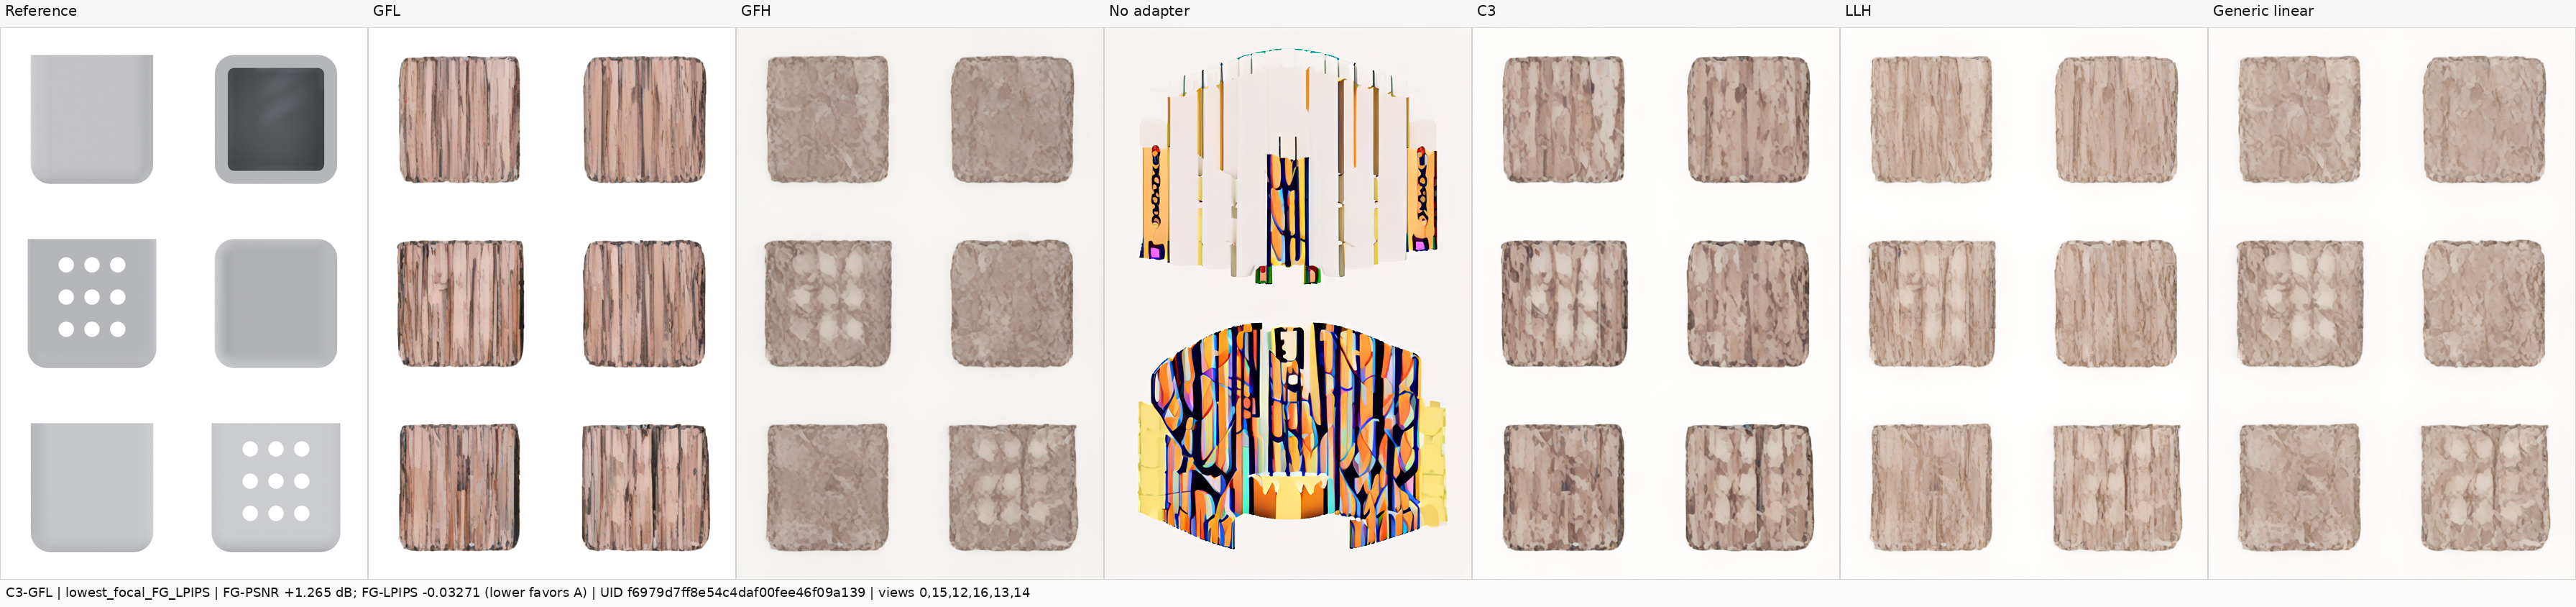
\includegraphics[width=\textwidth,trim=0 36pt 0 0,clip]{figures/figS1_color_detail_failure.png}
\caption{Selected illustrative failure cases from the rights-cleared Fresh C 2D pool. They are not representative estimates and do not support PBR, seam, or human-preference claims.}
\label{fig:supp-failures}
\end{figure}

The attempted Fresh C 24-object GLB bake did not pass its input/output gate: 9/24 sources had out-of-range native UVs, and 5 assets / 27 primitives used unsupported BLEND. No valid Fresh C 24-object bake results were generated. The seam endpoint is retired because the required seam truth set and native full-panel validation did not pass. No full PBR comparison is available. These checks are limitations, not evidence of method failure or success.

\section*{S8. Statistical authority and reproduction map}
Each numerical result in this Supplement is mapped to the internal claim ledger and scoped result sources. Fresh C primary contrasts use object-level deltas and a locked analysis; requested/applied-scale records use the per-step accounting table. Layer/window and Fresh B results are maintained in separate source summaries, with Fresh B classified as retrospective sensitivity because its lock chronology cannot be authenticated from preserved Git history. The texture-complexity cohort and the color-diagnostic set are separate from Fresh C and from each other. The historical N=20 GLB-native summary has a separate analysis record; no N=20 image assets are redistributed. Original Table 9 and Table 3 below are reproduced only as historical source text with explicit provenance limits; neither is treated as a newly verified current result.

\paragraph{Fresh C identity details.} The 300-object Fresh C list is disjoint by UID from the original eval300, including the 24-object development probe, the 1,118-object training list, and the clean-v2 eval300. The primary four-condition run and same-cohort Generic Linear/LLH addendum use the same frozen checkpoint SHA-256 \texttt{0618d6b2\allowbreak{}84ab47aa\allowbreak{}16d7a89d\allowbreak{}c447f5ba\allowbreak{}4455ff6c\allowbreak{}9d918e5e\allowbreak{}129478a9\allowbreak{}9e0114c0}, runner source SHA-256 \texttt{e5c28e915ba137d3541eb4c032daaf62a798332d63b32917b749fe1bcc74e9e3}, cohort, input tensors, endpoint implementation, and seed policy. The seed is $42+\texttt{object\_idx}$ and is shared across the matched conditions for each object. Primary and addendum integrity gates pass for 1,200/1,200 and 600/600 condition rows. Fresh C uses the recorded deep/middle/shallow caps of 3.0/3.5/0.8, with requested, applied, and residual scales logged separately. This is a held-out paired comparison under the stated protocol. The historical identity remains explicit: 01549 names v1 weights for its main tables and a separate v2 strong-residual, per-layer-capped instance for Section 4.7/FAC. Fresh C uses a controlled retraining and is not presented as a numerical reproduction of the old Table 4 $+0.96$ dB estimate.
\section*{S9. Historical 01549 Table 9: strict-276 schedule transfer}

The 01549 submission reports this schedule-transfer comparison on the 276 objects disjoint from the 24-object probe. It uses the strong-residual, per-layer-capped v2 adapter, not the v1 checkpoint named for 01549 Table 4. The values below are reproduced from the authenticated 01549 submission; they are not pooled with Fresh C or the separate MAIN-STAGE-276 profile-placement analysis. The table therefore documents schedule transfer on its stated adapter instance and remains distinct from Fresh C's matched single-checkpoint comparison.

\begin{table}[ht]
\centering\small
\caption{Values reproduced from original 01549 Table 9 for the stated strict-276 retrospective schedule-transfer comparison. The adapter/run differs from Fresh C; row-level runner and input provenance are incomplete. Values are preserved as submitted historical results, not independently verified statistics.}
\label{tab:historical-table9}
\begin{tabular}{lcccc}
\toprule
Schedule & FG-SSIM & PSNR & C3--schedule $\Delta$PSNR (95\% CI) & C3-favourable objects \\
\midrule
Trapezoid & 0.356 & 19.04 & $+0.258$ $[+0.207,+0.308]$ & 206/276 \\
Gaussian peak & 0.358 & 18.97 & $+0.324$ $[+0.281,+0.367]$ & 232/276 \\
Linear warm-up & 0.377 & 18.97 & $+0.323$ $[+0.263,+0.386]$ & 214/276 \\
Cosine bump & 0.330 & 18.39 & $+0.902$ $[+0.824,+0.981]$ & 253/276 \\
C3 (TCAS) & 0.376 & 19.29 & -- & -- \\
\bottomrule
\end{tabular}
\end{table}

\section*{S10. Historical 01549 Table 3: extended 24-object development diagnostics}

The table below is transcribed from the authenticated 01549 source and moved from the main text to preserve the original 24-object development record. The candidate-level row outputs and selection-time provenance are unavailable for independent reanalysis. Laplacian variance, RGB standard deviation, gradient magnitude, and high-frequency energy are variation diagnostics; this historical table does not establish texture fidelity, a population effect, or an optimal schedule.

\begin{table}[ht]
\centering\small
\caption{Values transcribed from original 01549 Table 3 for representative variants in the 24-object development probe. These are historical values, not independently recomputed statistics; variation measures do not establish texture fidelity.}\label{tab:historical-table3}
\begin{tabular}{lcccc}
\toprule
Variant & $\Delta$Lap Var & $\Delta$RGB Std & $\Delta$Grad & $\Delta$HF Energy \\
\midrule
C3 & $-$0.001 & $-$0.023 & +0.142 & +0.058 \\
C4 & $-$0.012 & $-$0.032 & +0.086 & +0.062 \\
A\_s2.50 & $-$0.011 & $-$0.044 & +0.054 & +0.078 \\
A\_s2.00 & $-$0.006 & $-$0.040 & +0.100 & +0.070 \\
A\_s1.25 & $-$0.005 & $-$0.032 & +0.104 & +0.053 \\
\bottomrule
\end{tabular}
\end{table}


\section*{S11. First-round FAC controlled re-examination}
The 01549 first-round package reports seven trained FAC configurations under the paired 300-object protocol. All values below are retained as originally reported; this is not a new 1008 training run. The 12-object untrained C3-envelope control is separate and is described in the main text.

\begin{longtable}{p{3.3cm}p{3.5cm}rrrr}
\caption{FAC dose-response table reported in the first-round 01549 supplement. FG-PSNR and FG-SSIM are the reported absolute values; $\Delta$FG-PSNR and wins compare each trained configuration with TCAS.}\label{tab:fac-dose-response}\\
\toprule
Configuration & Temporal gate & FG-PSNR & FG-SSIM & $\Delta$FG-PSNR & Wins \\
\midrule\endfirsthead
\toprule
Configuration & Temporal gate & FG-PSNR & FG-SSIM & $\Delta$FG-PSNR & Wins \\
\midrule\endhead
TCAS baseline (C3) & fixed C3 & 9.88 & 0.3681 & -- & -- \\
LTAG only & joint, unconstrained & 7.79 & 0.3487 & $-2.08$ & 4/300 \\
LTAG+GSG & joint, unconstrained & 7.03 & 0.3163 & $-2.84$ & 6/300 \\
Full FAC & joint, unconstrained & 6.94 & 0.3204 & $-2.94$ & 5/300 \\
Two-stage + GSG/FSC & frozen at C3 & 7.32 & 0.3074 & $-2.56$ & 4/300 \\
Envelope penalty ($\lambda=1$) & joint, penalized to C3 & 7.14 & 0.3021 & $-2.74$ & 2/300 \\
Fidelity weighting & frozen at C3 & 7.51 & 0.3110 & $-2.37$ & 5/300 \\
Gentle schedule & frozen at C3 & 8.77 & 0.4175 & $-1.10$ & 48/300 \\
\bottomrule
\end{longtable}

The submitted protocol states that only the LTAG/GSG/FSC controllers (roughly $6\times10^3$ parameters) were trained; the base model, VAE, and GeoTex-Adapter remained frozen. It specifies the enhanced latent denoising objective, AdamW, peak learning rate $10^{-4}$, 100 warm-up steps, and 2,000 training steps on a training pool stated as 1,706 objects and disjoint from the 300-object evaluation set. The 12-object untrained warm-start control was reported at $\Delta$FG-PSNR $=-0.18$ dB, 95\% CI [$-0.42,+0.05$]. A current archive audit found a recovered configuration listing 1,200 training objects and no run-bound seed/output manifest. The original result is therefore retained as reported in 01549 with this reproducibility limitation disclosed; no code-release claim is made.

\section*{S12. Retrospective texture-complexity boundary}
This analysis uses the separate FRESH\_CONFIRM\_300 cohort ($N=300$), not Fresh C or Fresh B. LLH and native GFL rows match the frozen object list and share the recorded checkpoint, runner, seed, six unique target views, sampler, and protocol. The paired LLH--GFL mean differences are $+1.2877$ dB FG-PSNR (95\% object-bootstrap CI [$+0.9383,+1.6346$]; 57.7\% LLH-favorable objects) and $-0.01650$ FG-LPIPS ([$-0.01887,-0.01413$]; 73.3\% LLH-favorable objects).

The descriptor analysis tests two image-space outcomes against five ground-truth descriptors: foreground Laplacian variance, RGB standard deviation, gradient magnitude, high-frequency energy, and coverage. Spearman correlations use average ranks and paired-object percentile bootstrap intervals (10,000 resamples, seed 20261002). The family contains ten plus-one-corrected bootstrap sign tests and Holm correction across all ten. Nine tests reject at 0.05; the only non-rejection is FG-LPIPS versus coverage (adjusted $p=0.0508$). The preserved H5 hypothesis excerpt predates one archived outcome bundle, but the main multiplicity lock classifies this family as retrospective after prior outcome exposure; that chronology has not been reconciled. We therefore report all associations as retrospective sensitivity evidence, not as preregistered confirmation.

\begin{table}[ht]
\centering\scriptsize
\caption{Retrospective Spearman associations between LLH--GFL image-space deltas and ground-truth descriptors in FRESH\_CONFIRM\_300. Correlation intervals are paired-object bootstrap intervals; adjusted $p$ values use the ten-test Holm family with plus-one-corrected bootstrap sign tests.}
\label{tab:texture-complexity}
\begin{tabular}{llrrl}
\toprule Outcome delta & Ground-truth descriptor & $\rho$ [95\% CI] & Holm $p$ & Decision \\
\midrule
FG-PSNR & Laplacian variance & $-0.524$ [$-0.603,-0.435$] & 0.0020 & reject \\
FG-PSNR & RGB standard deviation & $-0.380$ [$-0.488,-0.266$] & 0.0020 & reject \\
FG-PSNR & Gradient magnitude & $-0.464$ [$-0.548,-0.371$] & 0.0020 & reject \\
FG-PSNR & High-frequency energy & $-0.691$ [$-0.745,-0.626$] & 0.0020 & reject \\
FG-PSNR & Foreground coverage & $-0.134$ [$-0.241,-0.026$] & 0.0352 & reject \\
FG-LPIPS & Laplacian variance & $+0.604$ [$+0.511,+0.681$] & 0.0020 & reject \\
FG-LPIPS & RGB standard deviation & $+0.379$ [$+0.272,+0.482$] & 0.0020 & reject \\
FG-LPIPS & Gradient magnitude & $+0.563$ [$+0.469,+0.643$] & 0.0020 & reject \\
FG-LPIPS & High-frequency energy & $+0.677$ [$+0.599,+0.744$] & 0.0020 & reject \\
FG-LPIPS & Foreground coverage & $-0.118$ [$-0.233,+0.0002$] & 0.0508 & not rejected \\
\bottomrule
\end{tabular}
\end{table}

Ground-truth foreground Laplacian-variance quartiles contain 75 objects each. The FG-PSNR mean LLH--GFL difference declines from $+4.140$ dB in Q1 (92.0\% favor LLH) to $+1.127$ dB in Q2 (52.0\%), $-0.087$ dB in Q3 (41.3\%), and $-0.029$ dB in Q4 (45.3\%). The FG-LPIPS mean changes are $-0.03745$, $-0.01665$, $-0.00670$, and $-0.00520$ from Q1 to Q4; the favorable-object rates decline from 97.3\% to 50.7\%. These strata describe heterogeneity in this cohort. They do not establish that texture complexity causes the response, define a threshold, validate an object selector, or measure texture fidelity.

\section*{S13. Paired color-pathway diagnosis and failure boundaries}
The color diagnosis is a selected, failure-enriched set of 26 objects: six earlier figure cases and 20 Fresh C panels. It is not a random sample, a new holdout, or a population estimate. No Adapter, GFL, and LLH were compared on the same object inputs, checkpoint and runner, with six unique target views per object (78 object-condition records). CIEDE2000 and color-difference components were recomputed from hash-identified RGB images and frozen foreground masks. The object-level intervals below are paired percentile bootstrap intervals (20,000 resamples, seed 61008); they are descriptive and no confirmatory multiplicity family was defined for this diagnostic.

\begin{table}[ht]
\centering\scriptsize
\caption{Selected paired endpoints from the failure-enriched 26-object color diagnosis. Each row is condition A minus B with an object-level 95\% paired-bootstrap CI. Lower CIEDE2000 and FG-LPIPS are favorable; higher PSNR and Edge-SSIM are favorable. Local texture statistics describe variation, not fidelity.}
\label{tab:color-diagnostic}
\begin{tabular}{llrr}
\toprule Contrast & Endpoint & Mean difference & 95\% CI \\
\midrule
GFL -- No Adapter & Foreground CIEDE2000 & $-19.654$ & [$-26.370,-13.248$] \\
GFL -- No Adapter & FG-PSNR (dB) & $+6.646$ & [$+5.556,+7.635$] \\
GFL -- No Adapter & FG-LPIPS & $-0.03251$ & [$-0.05363,-0.01072$] \\
GFL -- No Adapter & Edge-SSIM & $+0.06510$ & [$+0.04853,+0.08202$] \\
LLH -- GFL & Foreground CIEDE2000 & $+3.583$ & [$+0.462,+6.712$] \\
LLH -- GFL & FG-PSNR (dB) & $-0.197$ & [$-1.562,+1.297$] \\
LLH -- GFL & FG-LPIPS & $-0.01294$ & [$-0.02742,+0.00066$] \\
LLH -- GFL & Edge-SSIM & $-0.00080$ & [$-0.00776,+0.00659$] \\
LLH -- GFL & Foreground gradient magnitude & $-0.06772$ & [$-0.08132,-0.05494$] \\
LLH -- GFL & Foreground high-frequency energy & $-0.00887$ & [$-0.01091,-0.00672$] \\
LLH -- GFL & Foreground color entropy & $-0.598$ & [$-0.703,-0.502$] \\
\bottomrule
\end{tabular}
\end{table}

GFL lowered reference-relative CIEDE2000 in 24/26 objects, yet the two original Figure~4 cases retained pink or purple shifts under No Adapter, GFL, and LLH. LLH had higher mean CIEDE2000 and lower gradient, high-frequency energy, and color entropy than GFL; these changes do not show improved fidelity. The decoded RGB showed pink before UV projection or baking, and a late denoising snapshot (update 40 of 50) showed it as well. On one selected case, a ground-truth VAE encode--decode isolate gave CIEDE2000 4.086 and $\Delta a^*\approx-1.35$, while GFL gave 22.032 and $+1.977$. This weakens ordinary VAE round-trip error as the sole explanation but does not identify the complete cause.

A feature-relative residual gate was negative: versus C3 it increased mean CIEDE2000 by 1.35 across 26 objects and by 3.18 in the six earlier cases, with no clear visual reduction in pink shift. No further repair search was started because no causal control point was identified. No complete cause or validated repair is established.

\end{document}
